% Standalone TikZ figure: Path Tracing vs Rasterization Rendering Comparison
% For Chapter 4: Synthetic Data Generation for Object Detection
\documentclass[tikz,border=10pt]{standalone}
\usepackage{tikz}
\usetikzlibrary{arrows.meta, positioning, shapes.geometric, fit, backgrounds, calc, patterns}

\begin{document}
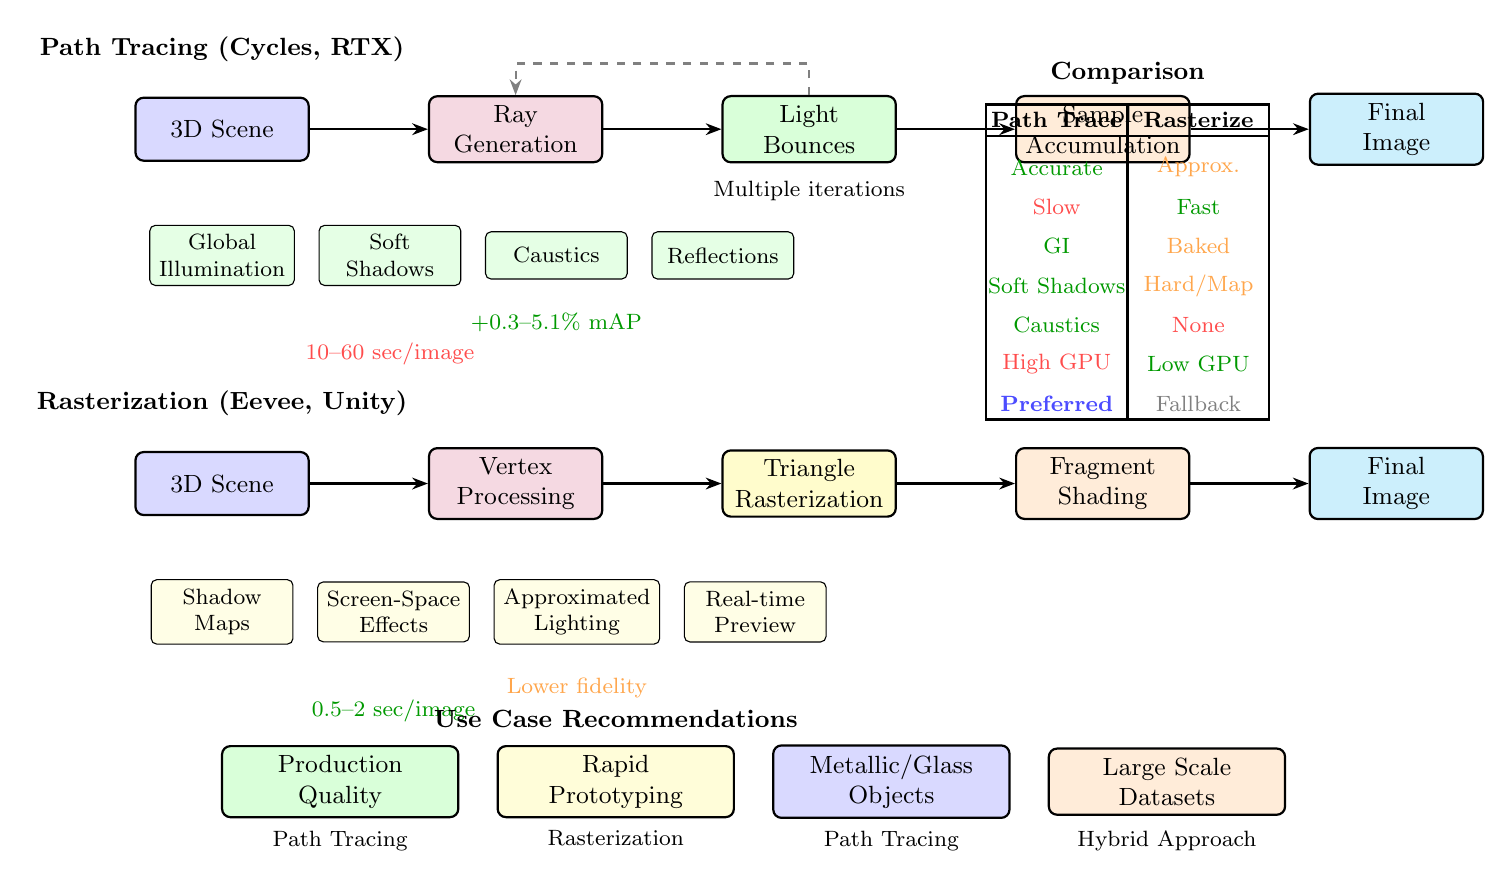
\begin{tikzpicture}[
    every node/.style={font=\small},
    box/.style={rectangle, draw, thick, minimum width=2.2cm, minimum height=0.8cm, align=center, rounded corners=3pt},
    smallbox/.style={rectangle, draw, minimum width=1.8cm, minimum height=0.6cm, align=center, rounded corners=2pt, font=\footnotesize},
    arrow/.style={-{Stealth[length=2mm]}, thick},
    label/.style={font=\footnotesize},
    title/.style={font=\bfseries\small}
]

% ============ PATH TRACING (TOP) ============
\node[title] at (0, 0) {Path Tracing (Cycles, RTX)};

% Scene
\node[box, fill=blue!15, below=0.6cm of {(0,0)}] (pt_scene) {3D Scene};

% Ray generation
\node[box, fill=purple!15, right=1.5cm of pt_scene] (pt_rays) {Ray\\Generation};

% Bounces
\node[box, fill=green!15, right=1.5cm of pt_rays] (pt_bounce) {Light\\Bounces};
\node[label, below=0.1cm of pt_bounce] {Multiple iterations};

% Accumulation
\node[box, fill=orange!15, right=1.5cm of pt_bounce] (pt_accum) {Sample\\Accumulation};

% Output
\node[box, fill=cyan!20, right=1.5cm of pt_accum] (pt_out) {Final\\Image};

% Arrows
\draw[arrow] (pt_scene) -- (pt_rays);
\draw[arrow] (pt_rays) -- (pt_bounce);
\draw[arrow] (pt_bounce) -- (pt_accum);
\draw[arrow] (pt_accum) -- (pt_out);

% Bounce loop
\draw[arrow, dashed, gray] (pt_bounce.north) -- ++(0,0.4) -| (pt_rays.north);

% Features
\node[smallbox, fill=green!10, below=0.8cm of pt_scene] (pt_f1) {Global\\Illumination};
\node[smallbox, fill=green!10, right=0.3cm of pt_f1] (pt_f2) {Soft\\Shadows};
\node[smallbox, fill=green!10, right=0.3cm of pt_f2] (pt_f3) {Caustics};
\node[smallbox, fill=green!10, right=0.3cm of pt_f3] (pt_f4) {Reflections};

% Performance annotation
\node[label, text=red!70, below=0.6cm of pt_f2] {10--60 sec/image};
\node[label, text=green!60!black, below=0.3cm of pt_f3] {+0.3--5.1\% mAP};

% ============ RASTERIZATION (BOTTOM) ============
\node[title] at (0, -4.5) {Rasterization (Eevee, Unity)};

% Scene
\node[box, fill=blue!15, below=0.6cm of {(0,-4.5)}] (rs_scene) {3D Scene};

% Vertex processing
\node[box, fill=purple!15, right=1.5cm of rs_scene] (rs_vertex) {Vertex\\Processing};

% Rasterization
\node[box, fill=yellow!20, right=1.5cm of rs_vertex] (rs_raster) {Triangle\\Rasterization};

% Fragment
\node[box, fill=orange!15, right=1.5cm of rs_raster] (rs_frag) {Fragment\\Shading};

% Output
\node[box, fill=cyan!20, right=1.5cm of rs_frag] (rs_out) {Final\\Image};

% Arrows
\draw[arrow] (rs_scene) -- (rs_vertex);
\draw[arrow] (rs_vertex) -- (rs_raster);
\draw[arrow] (rs_raster) -- (rs_frag);
\draw[arrow] (rs_frag) -- (rs_out);

% Features
\node[smallbox, fill=yellow!10, below=0.8cm of rs_scene] (rs_f1) {Shadow\\Maps};
\node[smallbox, fill=yellow!10, right=0.3cm of rs_f1] (rs_f2) {Screen-Space\\Effects};
\node[smallbox, fill=yellow!10, right=0.3cm of rs_f2] (rs_f3) {Approximated\\Lighting};
\node[smallbox, fill=yellow!10, right=0.3cm of rs_f3] (rs_f4) {Real-time\\Preview};

% Performance annotation
\node[label, text=green!60!black, below=0.6cm of rs_f2] {0.5--2 sec/image};
\node[label, text=orange!70, below=0.3cm of rs_f3] {Lower fidelity};

% ============ COMPARISON TABLE ============
\begin{scope}[shift={(11.5, -2.5)}]
    \node[title] at (0, 2.2) {Comparison};

    % Table
    \draw[thick] (-1.8, 1.8) rectangle (1.8, -2.2);
    \draw[thick] (-1.8, 1.4) -- (1.8, 1.4);
    \draw[thick] (0, 1.8) -- (0, -2.2);

    % Headers
    \node[font=\footnotesize\bfseries] at (-0.9, 1.6) {Path Trace};
    \node[font=\footnotesize\bfseries] at (0.9, 1.6) {Rasterize};

    % Rows
    \node[font=\footnotesize, text=green!60!black] at (-0.9, 1.0) {Accurate};
    \node[font=\footnotesize, text=orange!70] at (0.9, 1.0) {Approx.};

    \node[font=\footnotesize, text=red!70] at (-0.9, 0.5) {Slow};
    \node[font=\footnotesize, text=green!60!black] at (0.9, 0.5) {Fast};

    \node[font=\footnotesize, text=green!60!black] at (-0.9, 0.0) {GI};
    \node[font=\footnotesize, text=orange!70] at (0.9, 0.0) {Baked};

    \node[font=\footnotesize, text=green!60!black] at (-0.9, -0.5) {Soft Shadows};
    \node[font=\footnotesize, text=orange!70] at (0.9, -0.5) {Hard/Map};

    \node[font=\footnotesize, text=green!60!black] at (-0.9, -1.0) {Caustics};
    \node[font=\footnotesize, text=red!70] at (0.9, -1.0) {None};

    \node[font=\footnotesize, text=red!70] at (-0.9, -1.5) {High GPU};
    \node[font=\footnotesize, text=green!60!black] at (0.9, -1.5) {Low GPU};

    \node[font=\footnotesize\bfseries, text=blue!70] at (-0.9, -2.0) {Preferred};
    \node[font=\footnotesize, text=gray] at (0.9, -2.0) {Fallback};
\end{scope}

% ============ USE CASE RECOMMENDATIONS ============
\begin{scope}[shift={(0, -9)}]
    \node[title] at (5, 0.5) {Use Case Recommendations};

    \node[box, fill=green!15, minimum width=3cm] at (1.5, -0.3) {Production\\Quality};
    \node[label, below=0.1cm of {(1.5, -0.7)}] {Path Tracing};

    \node[box, fill=yellow!15, minimum width=3cm] at (5, -0.3) {Rapid\\Prototyping};
    \node[label, below=0.1cm of {(5, -0.7)}] {Rasterization};

    \node[box, fill=blue!15, minimum width=3cm] at (8.5, -0.3) {Metallic/Glass\\Objects};
    \node[label, below=0.1cm of {(8.5, -0.7)}] {Path Tracing};

    \node[box, fill=orange!15, minimum width=3cm] at (12, -0.3) {Large Scale\\Datasets};
    \node[label, below=0.1cm of {(12, -0.7)}] {Hybrid Approach};
\end{scope}

\end{tikzpicture}
\end{document}
